% Created 2023-08-25 Fri 12:04
% Intended LaTeX compiler: pdflatex
\documentclass[10pt, a4paper, twoside, headinclude,footinclude, BCOR5mm]{scrartcl}
\usepackage[utf8]{inputenc}
\usepackage[T1]{fontenc}
\usepackage{graphicx}
\usepackage{longtable}
\usepackage{wrapfig}
\usepackage{rotating}
\usepackage[normalem]{ulem}
\usepackage{amsmath}
\usepackage{amssymb}
\usepackage{capt-of}
\usepackage{hyperref}
\usepackage[nochapters, beramono, eulermath, pdfspacing, dottedtoc]{classicthesis}
\usepackage{arsclassica}
\usepackage[T1]{fontenc}
\usepackage[utf8]{inputenc}
\usepackage{amsmath,amssymb,amsthm}
\DeclareMathOperator{\erfc}{erfc}
\usepackage{enumitem}
\usepackage{parskip}
\usepackage{tcolorbox}
\usepackage{listings}
\definecolor{light-gray}{gray}{0.95} %the shade of grey that stack exchange uses
\publishers{\normalsize{University of Twente, Faculty of Engineering Technology \\ Mechanics of Solids, Surfaces and Systems, Chair of Production Technology}}
\author{Wouter Grouve}
\date{}
\title{THERMESH\\\medskip
\large A simple FE code for 1D heat conduction}
\hypersetup{
 pdfauthor={Wouter Grouve},
 pdftitle={THERMESH},
 pdfkeywords={Conduction, FE, Derivation},
 pdfsubject={},
 pdfcreator={Emacs 29.1 (Org mode 9.6.6)}, 
 pdflang={English}}
\begin{document}

\maketitle


\section{Introduction}
\label{sec:org5e87da7}

The present document presents the derivation of a element code for one dimensional transient heat conduction problems using both linear and quadratic elements. The code has been implemented in a Python package called \texttt{thermesh} is available for download from the author's Github page. Three validation cases are presented at the end of this document to show that the code is implemented correctly. Further, the validation cases can be used as examples and inspiration.

\section{Derivation}
\label{sec:org7b8095b}

\subsection{Governing partial differential equation and weak form}
\label{sec:org48b3671}

In the case of 1D heat conduction, the governing partial differential equation reads:
\begin{equation}
  \rho c_\text{p}\frac{\partial T}{\partial z} -
  k\frac{\partial^2 T}{\partial z^2} -
  \dot{Q} = 0
  \label{eq:pde}
\end{equation}
with \(T(z,t)\) the temperature at location \(z\) and time \(t\), \(\rho c_{\text{p}}\) the volumetric heat capacity, \(k\) the thermal conductivity, and \(\dot{Q}\) an internal  source or sink, e.g. due to a phase transformation. The partial differential equation is subject to boundary conditions at the two ends of the domain, which can be of the Dirichlet type:
\begin{equation*}
  T(0,t) = T_\text{left}(t), \qquad T(L,t) = T_\text{right}(t),
\end{equation*}
or of the Neumann type:
\begin{equation*}
  -k_{\text{z}}\frac{\partial T}{\partial z}\Biggr|_{z=0} = q_\text{left}(t), \qquad
  -k_{\text{z}}\frac{\partial T}{\partial z}\Biggr|_{z=L} = q_{\text{right}}(t),
\end{equation*}
with \(T_\text{left}\) and \(T_\text{right}\) an imposed temperature and \(q_\text{left}\) and \(q_\text{right}\) an imposed heat flux density. The latter could be either directly imposed \(\hat{q}\), for example as a result of laser heating, or be the result of convection:
\begin{equation*}
  q = h(T_{\infty}-T),
\end{equation*}
in which \(h\) and \(T_{\infty}\) are the heat transfer coefficient and the far field temperature, or the result of thermal radiation:
\begin{equation*}
  q = \epsilon\sigma(T_{\infty}^4-T^4),
\end{equation*}
where \(\epsilon\) is the surface emissivity and \(\sigma\) is Stefan's constant.

We can approximate the solution \(T(z,t)\) of the partial differential equation using the weighted residual method:
\begin{equation}
  \int_L w\left(
  \rho c_\text{p} \frac{\partial T}{\partial t} -
  k \frac{\partial^2 T}{\partial z^2} -
  \dot{Q} \right) \text{d}z = 0,
  \label{eq:weighted_residual}
\end{equation}
with \(w\) a weighting function.


\subsection{Discretization in space}
\label{sec:org24ee86a}

The domain in \(N\) is now split up in smaller elements, as is indicated in Figure \ref{fig:org64cda58} which shows an element \((e)\) of length \(\ell\) that is bounded by the nodes \(i\) and \(j\). The weighted residual (Equation \ref{eq:weighted_residual}) can now be rewritten as:
\begin{equation}
  \sum_{e=1}^N
  \int_\ell w\left(
    \rho c_\text{p}\frac{\partial T}{\partial t} -
    k\frac{\partial^2 T}{\partial z^2} -
    \dot{Q} \right) \text{d}z = 0.
    \label{eq:weighted_residual_sum}
\end{equation}
We will now make sure that the weighted residual vanishes for each element. Further, we get rid of the second derivative with respect to \(z\) in the second term using integration by parts:
\begin{equation*}
  \int_\ell w \rho c_\text{p}\frac{\partial T}{\partial t} \text{d}z +
  \int_\ell
  \frac{\text{d}w}{\text{d}z}k\frac{\partial T}{\partial z}\text{d}z -
  wk\frac{\partial T}{\partial z}\Biggr|_{z_i}^{z_j} -
  \int_\ell w \dot{Q} \text{d}z = 0,
\end{equation*}
with \(z_i\) and \(z_j\) the element end points. Realizing that the third term represents the flux (\(q = -k \partial T / \partial z\)), the equation can be rewritten as:
\begin{equation}
  \int_\ell w \rho c_\text{p}\frac{\partial T}{\partial t} \text{d}z +
  \int_\ell
  \frac{\text{d}w}{\text{d}z}k\frac{\partial T}{\partial z}\text{d}z
  = \int_\ell w \dot{Q} \text{d}z -
  w q \Biggr|_{z_i}^{z_j}.
  \label{eq:weighted_residual_el}
\end{equation}

\begin{figure}[!tb]
\centering
\includegraphics[width=12cm]{./fig/lin_elements_sf.png}
\caption{\label{fig:org64cda58}Left: Elements in 1D domain. Right: Definition of local coordinate system and linear interpolation of temperature.}
\end{figure}

\subsubsection{Linear shape functions}
\label{sec:orgb88bce0}

The temperature inside an element is approximated as a linear interpolation between the bounding node temperatures as:
\begin{equation}
  T(\zeta) = N_i(\zeta)T_i + N_j(\zeta)T_j,
  \label{eq:T_approx}
\end{equation}
with \(\zeta\) a local coordinate, as is illustrated in Figure \ref{fig:org64cda58}, defined as:
\begin{equation*}
  \zeta(z) = \frac{2z - (z_i + z_j)}{\ell},
\end{equation*}
while the two shape functions are:
\begin{equation}
  N_i(\zeta) = \frac{1-\zeta}{2} \quad\text{and}\quad
  N_j(\zeta) = \frac{1+\zeta}{2}.
  \label{eq:shape_functions}
\end{equation}
The spatial derivative of the temperature with respect to \(z\) can now be calculated as:
\begin{equation*}
  \frac{\partial T}{\partial z} =
  \frac{\partial T}{\partial \zeta}\frac{\partial \zeta}{\partial z},
\end{equation*}
with:
\begin{equation*}
  \frac{\partial \zeta}{\partial z} = \frac{2}{\ell}
  \quad\text{and}\quad
  \frac{\partial T}{\partial \zeta} = \frac{T_j - T_i}{2},
\end{equation*}
such that:
\begin{equation}
  \frac{\partial T}{\partial z} = \frac{T_j - T_i}{\ell},
  \label{eq:dTdz}
\end{equation}
which intuitively makes sense. Further, noting that the shape functions do not depend on time, we can rewrite the time derivative as:
\begin{equation}
  \frac{\partial T}{\partial t} =
  N_i(\zeta)\frac{\partial T_i}{\partial t} +
  N_j(\zeta)\frac{\partial T_j}{\partial t}.
  \label{eq:dTdt}
\end{equation}

Following the Galerkin method, we choose our weighting function \(w\) to be our shape functions. The equation for the weighted residual for an element (Equation \ref{eq:weighted_residual_el}) can now be rewritten as:
\begin{equation}
  \int_\ell N_k \rho c_\text{p}\frac{\partial T}{\partial t} \text{d}z +
  \int_\ell
  \frac{\text{d}N_k}{\text{d}z}k\frac{\partial T}{\partial z}\text{d}z  =
  \int_\ell N_k \dot{Q} \text{d}z - N_k q \Biggr|_{z_i}^{z_j}
  \quad\text{for: } k = 1,2.
  \label{eq:galerkin}
\end{equation}
with \(N_k\) the two shape functions as defined in Equation \ref{eq:shape_functions}.

\begin{tcolorbox}[colback=gray!5,colframe=gray!40!black,title=Matrix-vector notation]
Before evaluating the integrals, we first rewrite the expressions from the previous section into a matrix-vector form. Starting with Equation \ref{eq:T_approx}, which can be written as:
\begin{equation*}
  T(\zeta) = \mathbf{N}\mathbf{T},
\end{equation*}
in which:
\begin{equation*}
\mathbf{N} = [N_i(\zeta), N_j(\zeta)] \quad\text{and}\quad
\mathbf{T} = \begin{Bmatrix} T_i \\ T_j \end{Bmatrix} \,
\end{equation*}
The spatial derivative of the temperature (Equation \ref{eq:dTdz}) yields:
\begin{equation*}
  \frac{\partial T}{\partial z} =
  \frac{\partial T}{\partial \zeta}\frac{\partial \zeta}{\partial z} =
  \frac{2}{\ell}\frac{\partial\mathbf{N}\mathbf{T}}{\partial \zeta} =
  \frac{2}{\ell}\frac{\partial \mathbf{N}}{\partial\zeta} \mathbf{T} =
  \mathbf{B}\mathbf{T},
\end{equation*}
with:
\begin{equation*}
  \mathbf{B} = \frac{2}{\ell}\frac{\partial \mathbf{N}}{\partial\zeta}= \frac{2}{\ell}
  \left[\frac{\partial N_i}{\partial \zeta}, \frac{\partial N_j}{\partial \zeta}\right] =
  \left[-\frac{1}{\ell}, \frac{1}{\ell}\right],
\end{equation*}
while the time-derivative of the temperature can be rewritten as:
\begin{equation*}
  \frac{\partial T}{\partial t} =
  \mathbf{N}\mathbf{\dot{T}}.
\end{equation*}
Further, for convenience, we will write our weighting functions as:
\begin{equation*}
  w = \mathbf{N}^T = \begin{Bmatrix} N_i \\ N_j \end{Bmatrix}.
\end{equation*}
\end{tcolorbox}

We can now evaluate the integrals, starting with the first term:
\begin{equation*}
  \int_\ell w \rho c_\text{p}\frac{\partial T}{\partial t} \text{d}z =
  \rho c_\text{p}\int_\ell \mathbf{N}^T \mathbf{N} \text{d}z \; \mathbf{\dot{T}}.
\end{equation*}
We can rewrite this integral in terms of \(\zeta\), by making use of the derivative of \(\zeta\) with respect to \(z\):
\begin{equation*}
  \frac{\text{d}\zeta}{\text{d}z} = \frac{2}{\ell} \quad\rightarrow\quad
  \text{d}z = \frac{\ell}{2}\text{d}\zeta,
\end{equation*}
such that:
\begin{equation}
\label{eq:C}
  \rho c_\text{p} \int_\ell \mathbf{N}^T \mathbf{N}\text{d}z \;\mathbf{\dot{T}} =
  \frac{\ell\rho c_\text{p}}{2}\int_{-1}^{1} \mathbf{N}^T \mathbf{N} \text{d}\zeta \; \mathbf{\dot{T}} =
  \mathbf{C}\mathbf{\dot{T}},
\end{equation}
with:
\begin{equation*}
  \mathbf{C} = \frac{\ell\rho c_\text{p}}{2}\int_{-1}^{1} \mathbf{N}^T\mathbf{N} \text{d}\zeta =
  \frac{\ell\rho c_\text{p}}{6}\left[\begin{matrix} 2 & 1\\
                                               1 & 2\end{matrix}\right].
\end{equation*}

In the same manner, the second term yields:
\begin{equation}
  \int_\ell \frac{\text{d}N_k}{\text{d}z}k\frac{\partial T}{\partial z}\text{d}z =
  \frac{\ell k}{2} \int_{-1}^{1} \mathbf{B}^T \mathbf{B} \text{d}\zeta \;\mathbf{T} = \mathbf{K} \mathbf{T},
  \label{eq:K}
\end{equation}
with:
\begin{equation*}
  \mathbf{K} = \frac{\ell k}{2} \int_{-1}^{1} \mathbf{B}^T \mathbf{B} \text{d}\zeta =
  \frac{k}{\ell}\left[\begin{matrix} 1 & -1\\
                                              -1 & 1\end{matrix}\right].
\end{equation*}

The first term on the right hand side yields:
\begin{equation*}
  \int_\ell \mathbf{N}^T \dot{Q} \text{d}z =
  \frac{\dot{Q}\ell}{2} \int_{-1}^{1} \mathbf{N}^T \text{d}\zeta   = \frac{ \dot{Q} \ell}{2} \begin{Bmatrix} 1 \\ 1 \end{Bmatrix},
\end{equation*}
with \(\dot{Q}\) the heat source term for the element between nodes \(i\) and \(j\). The second term, with the heat flux \(q\) on the boundary, is first expanded to include both a direct heat flux \(\hat{q}\) and a flux due to convection:
\begin{equation*}
  q = \hat{q} + h(T_{\infty}-T),
\end{equation*}
which yields:
\begin{equation*}
  N_k q \Biggr|_{z_i}^{z_j} = N_k \hat{q} \Biggr|_{z_i}^{z_j} +
                             N_k h (T_{\infty}-T) \Biggr|_{z_i}^{z_j}.
\end{equation*}
The term with the direct heat flux \(\hat{q}\) is evaluated as:
\begin{equation*}
  N_k \hat{q} \Biggr|_{z_i}^{z_j} =
     \begin{Bmatrix} N_i(z_j)q_j - N_i(z_i) \hat{q}_i \\
                     N_j(z_j)q_j - N_j(z_i) \hat{q}_i \end{Bmatrix} =
     \begin{Bmatrix} - \hat{q}_i \\
                       \hat{q}_j \end{Bmatrix},
\end{equation*}
with \(\hat{q}_k\) the heat flux on the \(k\)-th node. The convective term can be accounted for using a stiffness matrix for convection:
\begin{equation}
  N_k h T \Biggr|_{z_i}^{z_j} = \mathbf{H} \mathbf{T} \quad{with:}\quad
      \mathbf{H} = h\left[\begin{matrix} N_i N_i & N_i N_j \\
                                       N_j N_i & N_j N_j \end{matrix}\right],
\label{eq:H}
\end{equation}
and an additional term in the force vector:
\begin{equation*}
  N_k h T_{\infty} \Biggr|_{z_i}^{z_j} =
     h\begin{Bmatrix} - T_{\infty,i} \\
                        T_{\infty,j} \end{Bmatrix}.
\end{equation*}
As an example for the stiffness matrix \(\mathbf{H}\), in case of a convective boundary condition at the j-th node, where \(N_i = 0\), this term would evaluate as:
\begin{equation*}
  \mathbf{H} = \left[\begin{matrix} N_i N_i & N_i N_j \\
                                  N_j N_i & N_j N_j \end{matrix}\right] =
             \left[\begin{matrix} 0 & 0 \\
                                  0 & 1 \end{matrix}\right],
\end{equation*}
which intuitively makes sense. The force vector is now combined as:
\begin{equation}
\mathbf{f} = \int_\ell N_k \dot{Q} \text{d}z - N_k q \Biggr|_{z_i}^{z_j} -          N_k h T_{\infty} \Biggr|_{z_i}^{z_j} =
           \frac{\dot{Q}\ell}{2}\begin{Bmatrix} 1 \\ 1\end{Bmatrix} +
           \begin{Bmatrix}  \hat{q}_i \\
                            -\hat{q}_j \end{Bmatrix} +
           h\begin{Bmatrix}  T_{\infty,i} \\
                             -T_{\infty,j} \end{Bmatrix}.
\label{eq:f}
\end{equation}

The final element equation can now be assembled by substituting Equations \ref{eq:C}, \ref{eq:K}, \ref{eq:H} and \ref{eq:f} in Equation \ref{eq:galerkin}:
\begin{equation*}
\mathbf{C}\mathbf{\dot{T}} + (\mathbf{K} + \mathbf{H})\mathbf{T} = \mathbf{f}.
\end{equation*}

With the local damping and stiffness matrices determined for each element, we can assemble  the global matrices using the node locations and element connectivity  in the global system.

\subsubsection{Quadratic shape functions}
\label{sec:org6987193}

\begin{figure}[htbp]
\centering
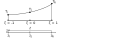
\includegraphics[width=6cm]{./fig/qua_elements_sf.png}
\caption{\label{fig:org68d459c}Definition of a regular local coordinate system and quadratic interpolation of temperature.}
\end{figure}

In the case of quadratic shape functions, the temperature inside an element is approximated as:
\begin{equation}
  T(\zeta) = N_i(\zeta)T_i + N_j(\zeta)T_j + N_k(\zeta)T_k,
  \label{eq:qua_interp}
\end{equation}
with reference to \ref{fig:org68d459c} for the node locations. The three shape functions are now defined as:
\begin{equation}
  N_i(\zeta) = -\frac{1}{2}\zeta (1-\zeta) \quad\text{and}\quad
  N_j(\zeta) = 1-\zeta^2 \quad\text{and}\quad
  N_j(\zeta) = \frac{1}{2}\zeta (1+\zeta),
  \label{eq:qua_shape_functions}
\end{equation}
or:
\begin{equation*}
  \mathbf{N} = \left[ -\frac{1}{2}\zeta (1-\zeta),
  1-\zeta^2,
  \frac{1}{2}\zeta (1+\zeta)\right].
\end{equation*}

The mapping between the local coordinate \(\zeta\) and the global coordinate \(x\) is achieved by:
\begin{equation*}
  z(\zeta) = N_i(\zeta)z_i + N_j(\zeta)z_j + N_i(\zeta)z_k.
\end{equation*}
Here, for convenience, we will consider a regular element which means that:
\begin{equation*}
  z_j = \frac{z_i + z_k}{2}.
\end{equation*}
The  Jacobian is now evaluated as:
\begin{equation*}
  \frac{\text{d}z}{\text{d}\zeta} = (\zeta - \frac{1}{2})z_i -
                                    2\zeta z_j +
                                    (\zeta + \frac{1}{2})z_k =
                                    \frac{\ell}{2}.
\end{equation*}
The temperature gradient with respect to \(z\) can be written as:
\begin{equation*}
  \frac{\text{d} T}{\text{d}z} =
  \frac{\text{d}\zeta}{\text{d}z} \frac{\partial T}{\partial \zeta} =
  \frac{2}{\ell}\frac{\partial \mathbf{N}}{\partial \zeta} \mathbf{T} =
  \mathbf{B}\mathbf{T},
\end{equation*}
with:
\begin{equation*}
\mathbf{B} = \frac{2}{\ell}\frac{\partial \mathbf{N}}{\partial\zeta}= \frac{2}{\ell}
\left[\frac{\partial N_i}{\partial \zeta}, \frac{\partial N_j}{\partial \zeta}, \frac{\partial N_k}{\partial \zeta}\right] =
\left[\frac{2\zeta - 1}{\ell}, -\frac{4\zeta}{\ell}, \frac{2\zeta + 1}{\ell}\right].
\end{equation*}

Now we can derive the damping matrix \(\mathbf{C}\) and the stiffness matrix \(\mathbf{K}\) in the same manner as we have done for the linear shape functions:
\begin{equation*}
  \mathbf{C} = \frac{\ell\rho c_\text{p}}{2}\int_{-1}^{1} \mathbf{N}^T\mathbf{N} \text{d}\zeta =
  \frac{\ell\rho c_\text{p}}{30}
  \left[\begin{matrix} 4 & 2 & -1\\
                       2 & 16 & 2 \\
                       -1 & 2 & 4\end{matrix}\right],
\end{equation*}
\begin{equation*}
  \mathbf{K} = \frac{\ell k}{2} \int_{-1}^{1} \mathbf{B}^T \mathbf{B} \text{d}\zeta =
  \frac{k}{3\ell}
  \left[\begin{matrix} 7 & -8 & 1\\
                       -8 & 16 & -8\\
                       1 & -8 & 7\end{matrix}\right],
\end{equation*}
while the term for the internal heat source \(\dot{Q}\) is evaulated as:
\begin{equation*}
  \frac{\dot{Q}\ell}{2} \int_{-1}^{1} \mathbf{N}^T \text{d}\zeta   = \frac{ \dot{Q} \ell}{6} \begin{Bmatrix} 1 \\ 4 \\ 1 \end{Bmatrix}.
\end{equation*}

\subsection{Temporal discretization}
\label{sec:orge6d0d6c}

The final step is to integrate the equation with respect to time. For this purpose, we will discretize the temporal variable using the so-called \(\Theta\)-method:
\begin{equation}
  \mathbf{C} \frac{\mathbf{T}_{\text{n}+1} - \mathbf{T}_\text{n}}{\Delta t} +
  (1-\Theta)(\mathbf{K}+\mathbf{H}) \mathbf{T}_{\text{n}} +
  \Theta(\mathbf{K}+\mathbf{H}) \mathbf{T}_{\text{n}+1}
  =
  (1-\Theta)\mathbf{f}_{\text{n}} + \Theta\mathbf{f}_{\text{n}+1},
  \label{eq:theta}
\end{equation}
with the subscript \(n\) denoting the time step, and where \(\Theta \in [0, 1]\). Common values of \(\Theta\) are:
\begin{eqnarray*}
  \Theta =& 0,   &\qquad\text{(Explit Euler)}\\
  \Theta =& 1/2, &\qquad\text{(Crank Nicolson)}\\
  \Theta =& 1,   &\qquad\text{(Implicit Euler)}.
\end{eqnarray*}
Equation \ref{eq:theta} can be rearranged as:
\begin{equation*}
  \Bigl( \mathbf{C} + \Delta t\Theta(\mathbf{K}+\mathbf{H})
  \Bigr) \mathbf{T}_{\text{n}+1} =
  \Bigl(
  \mathbf{C} - \Delta t(1-\Theta)(\mathbf{K}+\mathbf{H})
  \Bigr) \mathbf{T}_{\text{n}} +
  \Delta t(1-\Theta)\mathbf{f}_{\text{n}} +
  \Delta t\Theta\mathbf{f}_{\text{n}+1},
\end{equation*}
which can be solved to obtain the temperatures for each time step.

\section{Validation}
\label{sec:org50b76d1}

The finite elements derived here were  implemented in an object-oriented Python code called \texttt{thermesh}, which can be found on the author's \href{https://github.com/wjbg}{Github} page. Please note that, with the focus on readability, the code is far from optimized. Nevertheless, I believe it should still be more than fast enough for most problems. This section presents three short validation cases to show that the code is implemented correctly. Although all presented cases use linear elements, the code was also validated for the quadratic elements. Details on material properties and dimensions used for each case can be found in the respective Python files.

\subsection{Step temperature at boundary}
\label{sec:org14984d2}

Consider a domain of length \(L\) with a uniform initial temperature \(T_0\). For \(t>0\) the temperature at one end is raised to a value of \(T_{\text{end}}\), while the other end is kept at the initial temperature:
\begin{eqnarray*}
  T(x, 0) =& T_0\\
  T(0, t) =& T_0\\
  T(L, t) =& T_{\text{end}}.
\end{eqnarray*}
In case the initial temperature equals 0.0 \(^{\circ}\)C , the analytical solution\footnote{The Mathematics of Diffusion, Crank, 1975, pp 49-50.} yields:
\begin{equation*}
T(x,t) = \frac{T_{\text{end}}x}{L} + \frac{2}{\pi}
       \sum_{N=1}^{\infty} \frac{T_{\text{end}} \cos N\pi}{N}
       \sin\left(\frac{N\pi x}{L}\right)
       \exp\left(-\alpha N^2 \pi^2 t / L^2 \right),
\end{equation*}
with \(\alpha = k/\rho c_{\text{p}}\) the thermal diffusivity. The left graph in Figure \ref{fig:step_compare} shows the temperature distribution at different times. Code listing \ref{lst:step} illustrates how to solve this problem using \texttt{thermesh}. The right graph in Figure \ref{fig:step_compare} shows the finite element solution for 10 linear elements of equal length. Good comparison is obtained between the numerical and analytical solution. The code for this comparison is available in \texttt{step\_change.py}.

\lstset{basicstyle=\ttfamily}
\begin{minipage}{\linewidth}
\label{code:step}
\begin{lstlisting}[language=Python, caption=Thermesh example for a step change at one end., label={lst:step}, backgroundcolor=\color{light-gray}]
import numpy as np
import thermesh as tm

# Domain information
L = 0.01
k, rho, cp = 0.72, 1560, 1450
cpeek = tm.isothermal_model(k, rho, cp)  # constitutive model

# Mesh generation using linear elements
nn = 11  # number of nodes
z = np.linspace(0, L, nn)  # node locations
mesh = tm.Mesh(z, tm.LinearElement)

# Boundary conditions
bc = [{"T": 0.0},  # T on the left
      {"T": 1.0}]  # T on the right

# Domain generation and initialization
domain = tm.Domain(mesh, cpeek, bc)
domain.set_T(np.zeros(nn))

# Solve
solver = {"dt": 0.1, "t_end": 100.0, "theta": 0.5}  # settings
t, T = tm.solve_ht(domain, solver)
\end{lstlisting}
\end{minipage}

\begin{figure}[tbh]
\centering
\begin{minipage}{.5\textwidth}
  \centering
  \includegraphics[width=60mm]{fig/step_analytical_sol.png}
\end{minipage}%
\begin{minipage}{.5\textwidth}
  \centering
  \includegraphics[width=60mm]{fig/step_FE_t0.5_dt0.1s.png}
\end{minipage}
\caption{Comparison of the analytical and FE solution at different times for a step change in temperature at one end. The numbers in the graphs indicate the time in seconds.}
\label{fig:step_compare}
\end{figure}

\subsection{Constant heat flux at boundary of semi-infinite solid}
\label{sec:org842b196}

Consider a semi-infinite domain with a uniform initial temperature. The domain is subjected to a constant heat flux \(\hat{q}\) at the boundary which causes the temperature to increase:
\begin{eqnarray*}
  T(x, 0) =& T_0\\
  q(0, t) =& \hat{q}\\
  T(L, t) =& T_0.
\end{eqnarray*}
The analytical solution\footnote{Heat Transfer, Nillis \& Klein, 2008, p 362.} for the temperature increase \(\Delta T\) in the domain yields:
\begin{equation*}
T(x,t) - T_0(x,t) =
\Delta T(x,t) = \frac{\hat{q}}{k} \left[
                \sqrt{\frac{4\alpha t}{\pi}}
                \exp \left( -\frac{x^2}{4\alpha t} \right)-
                x \erfc \left( \frac{x}{2\sqrt{\alpha t}} \right)
                \right],
\end{equation*}
with \(\erfc\) the complementary error function. The left graph in \ref{fig:flux_compare} shows the temperature increase at 2, 10 and 25 seconds. Code listing \ref{lst:flux} illustrates the code to solve this problem using \texttt{thermesh}. Of course, one has to make sure that the domain is large enough (or the time short enough) for it to be considered a semi-infinite solid. The right graph in Figure \ref{fig:flux_compare} shows the finite element solution for 10 linear elements of equal length. Good comparison is obtained between the numerical and analytical solution. The code for this comparison is available in the Python file \texttt{constant\_heat\_flux.py}.

\lstset{basicstyle=\ttfamily}
\begin{minipage}{\linewidth}
\label{code:flux}
\begin{lstlisting}[language=Python, caption=Thermesh example for a constant heat flux at one end., label={lst:flux}, backgroundcolor=\color{light-gray}]
# Clear all solution data
domain.clear()

# Set new boundary conditions
bc = [{"q": 1E5},  # q on the left
      {"T": 0.0}]  # T on the right

# Solve
solver = {"dt": 0.1, "t_end": 25.0, "theta": 0.5}  # settings
t, T = tm.solve_ht(domain, solver)
\end{lstlisting}
\end{minipage}

\begin{figure}
\centering
\begin{minipage}{.5\textwidth}
  \centering
  \includegraphics[width=60mm]{fig/heatflux_analytical_sol.png}
\end{minipage}%
\begin{minipage}{.5\textwidth}
  \centering
  \includegraphics[width=60mm]{fig/heatflux_FE_t0.5_dt0.1s.png}
\end{minipage}
\caption{Comparison of the analytical and FE solution at different times in the case of a constant heat flux at one end. The numbers in the graphs indicate the time in seconds.}
\label{fig:flux_compare}
\end{figure}

\subsection{Convective boundary condition}
\label{sec:org9205675}

In the last example, we again consider a semi-infinite domain with a uniform initial temperature. The domain is now subjected to a convective boundary condition with a heat transfer coefficient \(h\) and a far field temperature \(T_{\infty}\).
\begin{eqnarray*}
  T(x, 0) =& T_0\\
  q(0, t) =& h(T_{\infty} - T(0,t))\\
  T(L, t) =& T_0.
\end{eqnarray*}
The analytical solution\footnote{See footnote 2.} for the temperature increase \(\Delta T\) in the domain yields:
\begin{equation*}
\Delta T(x,t) = (T_{\infty} - T_0)
                \left[\erfc\left( \frac{x}{2\sqrt{\alpha t}} \right) -
                \exp\left( \frac{hx}{k}+\frac{h^2 \alpha t}{k^2} \right)
                \erfc\left( \frac{x}{2\sqrt{\alpha t}} + \frac{h}{k}\sqrt{\alpha t} \right) \right].
\end{equation*}

The left graph in \ref{fig:conv_compare} shows the temperature increase at 2, 10 and 25 seconds. Code listing \ref{lst:conv} illustrates the code to solve this problem using \texttt{thermesh}. The right graph in Figure \ref{fig:conv_compare} shows the finite element solution for 10 linear elements of equal length. As can be seen, also here good comparison is obtained between the numerical and analytical solution. The code for this comparison is available in the Python file \texttt{convective\_bc.py}.

\lstset{basicstyle=\ttfamily}
\begin{minipage}{\linewidth}
\label{code:flux}
\begin{lstlisting}[language=Python, caption=Thermesh example for a constant heat flux at one end., label={lst:conv}, backgroundcolor=\color{light-gray}]
# Clear all solution data
domain.clear()

# Set new boundary conditions
bc = [{"h": 20,
       "T_inf": 400},  # h and T_inf on the left
      {"T": 0.0}]      # T on the right

# Solve
solver = {"dt": 0.1, "t_end": 25.0, "theta": 0.5}  # settings
t, T = tm.solve_ht(domain, solver)
\end{lstlisting}
\end{minipage}

\begin{figure}
\centering
\begin{minipage}{.5\textwidth}
  \centering
  \includegraphics[width=60mm]{fig/conv_analytical_sol.png}
\end{minipage}%
\begin{minipage}{.5\textwidth}
  \centering
  \includegraphics[width=60mm]{fig/conv_FE_t0.5_dt0.1s.png}
\end{minipage}
\caption{Comparison of the analytical and FE solution at different times in the case of a convective boundary condition at one end. The numbers in the graphs indicate the time in seconds.}
\label{fig:conv_compare}
\end{figure}
\end{document}